%! Author = NekoHitDev
%! Date = 2021/7/30
%! Language = English (US)
%! compiler = XeLaTex

% Preamble
\documentclass[12pt,a4paper]{article}
\usepackage[T1]{fontenc}

% Packages
\usepackage{amsmath}
\usepackage{url}
\usepackage{graphicx}
\usepackage[slantfont, boldfont]{xeCJK}

% set CJK font
\setCJKmainfont{SimSun}

% include header file
\newcommand{\editversion}{v0.0.1-RC1}

\newcommand{\gentitlepage}[1]{
    \begin{titlepage}
        \centering
        \vfill
        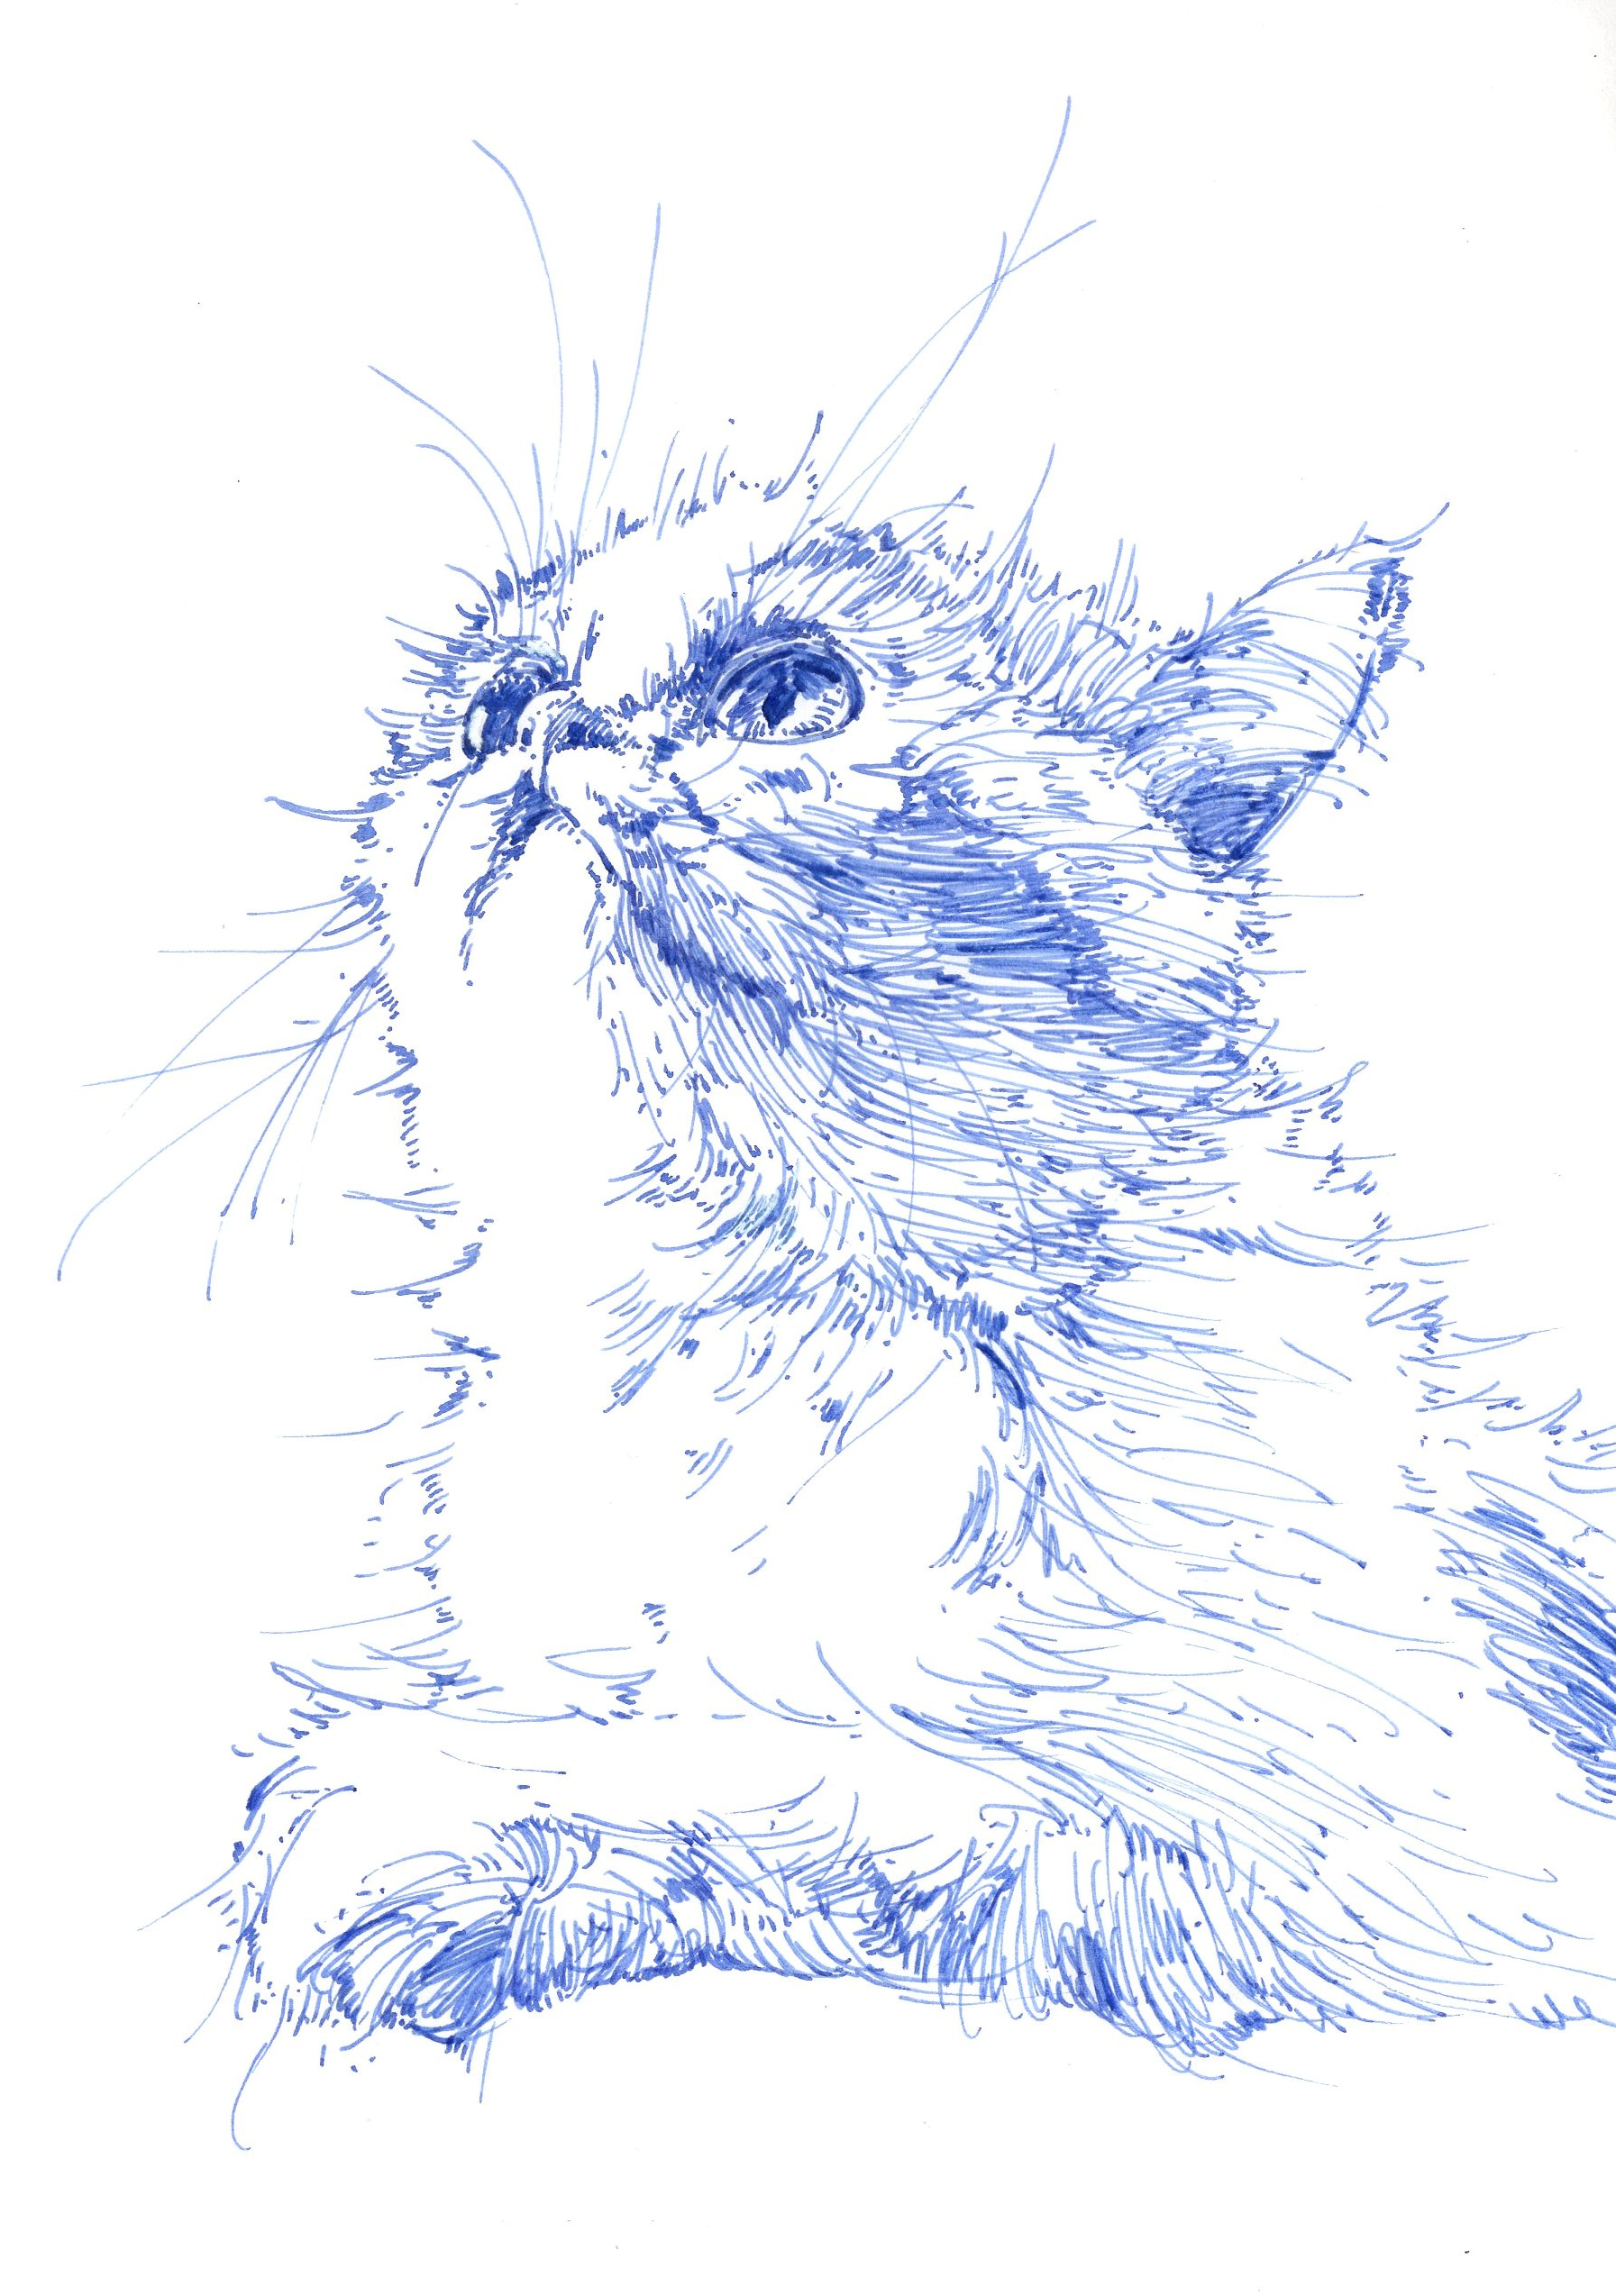
\includegraphics[width=0.8\textwidth]{assets/img196}
        \vfill
        {\Huge
        \textsf{NekoHit Project}\\
        #1\\
        \vskip2cm
        \vfill
        \Large
        \editversion
        }
        \vfill
        \vfill
    \end{titlepage}
}

% TOC stop at subsection
\setcounter{tocdepth}{2}


% Document
\begin{document}
    \gentitlepage{White paper}

    \thispagestyle{empty}
    \vspace*{\fill}
    \begin{center}
        \textit{To commemorate the author of the title pic, our friend, Uekawakuyuurei.}
    \end{center}
    \vspace*{\fill}
    \clearpage

    \pagenumbering{Roman}
    \tableofcontents
    \vspace*{\fill}
    \begin{center}
        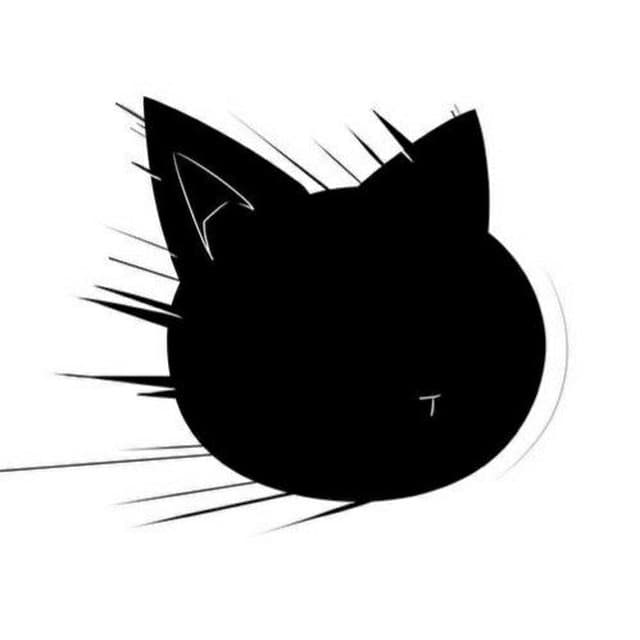
\includegraphics[width=0.67\textwidth]{assets/img197}
    \end{center}
    \clearpage

    \pagenumbering{arabic}


    \section{Vision of the future}\label{sec:goal}

    The vision (goal) of the NekoHit Project is to build a decentralized
    application that gives creators the freedom to spend their time and energy,
    and allows audiences to support creators financially while incentivizing
    creators to respond to sponsors.

    As more and more creators and sponsors join, we envisioned that the NekoHit
    community would grow and improve.
    We, the developers of this project, will respond to the needs and feedback
    from the community and strive to create an energetic platform for creators.


    \section{Introduction}\label{sec:intro}

    The NekoHit Project was built on top of the work completion agreement (WCA
    for short).
    The project aims to incorporate \textit{insurance} into the traditional sponsor
    model, promote audiences' willingness to support content creators financially,
    and motivate creators to comply with their promises and finish the project
    on time.

    The subscription model of the NekoHit Project is different from Patreon's.
    Instead of paying a monthly subscription fee, we allow the audience to sponsor
    a project more precisely.
    To gain the audience's trust, content creators need to pledge (stake) some
    tokens first.
    These tokens need to be transferred to our WCA smart contracts before the
    sponsors can transfer the tokens for sponsorship to the creator's projects.
    Our WCA contract also holds the sponsored tokens.
    When declaring a project, the creator needs to provide information such as
    the staking (pledging) rate, detailed milestones, and the expected completion
    time.
    Suppose the creator does not complete certain milestones by the scheduled time.
    In that case, the WCA contract will automatically calculate the percentage of
    those milestones to the project and deduct it from the pre-pledged tokens.
    After the project is completed, the deducted tokens will be released to each
    sponsor in proportion to the reference sponsorship amount.
    Also, tokens sponsored by sponsors will be deducted by the corresponding
    percentage and returned to the sponsor's wallet as a refund.
    So not only does the author not receive the sponsorship tokens for his defaulted
    milestone, but he also loses some of his own pledged tokens.

    We use this mechanism as a safety net to protect our sponsors' rights and
    incentivize creators to complete their projects in time.
    Such a mechanism will also urge the creators to think carefully about the
    project and arrange the timeline appropriately.
    Last but not least, we hope that this will increase the audience's trust in
    the content creators and reduce their concerns about financial sponsorship.


    \section{Industry Status}\label{sec:now}

    There is a growing interest in the creator economy, where audiences are
    willing to fund creators, and creators also need various sources of income
    to sustain their work.
    The market related to the creator economy is still relatively raw, which is
    undoubtedly an opportunity for us to grow.

    \subsection{Subscription-based traditional model}\label{subsec:tradition_patreon}

    The most typical of the traditional subscription-based model is Patreon.
    It is based on a monthly subscription model, where creators can customize
    their plans at different prices.
    Usually, the lower price means fewer returns.
    Take the famous illustrator WLOP as an example.
    His Patreon has five plans\cite{wlop_patreon}:
    \begin{itemize}
        \item Knight: \$2 per month, with JPG format comics (3000 pixels wide)
        and wallpaper created that month (4K resolution)
        \item Black Knight: \$4 per month, with full-size comic and the wallpaper
        created that month (8K resolution)
        \item Templar: \$8 per month, with everything in Black Knight and brushes
        used by WOLP in Photoshop and PSD source files created that month.
        \item Angel: \$14 per month, with everything in the Templar, discounts
        in WLOP's store, and other bonus that help you learn painting.
        \item Asura: \$20 per month, with everything in Angel. And free
        access to one of the source files of any previous works, tutorials, or
        dynamic wallpapers per month.
    \end{itemize}\footnote{
        WLOP's Patreon is charged in the term, two terms per month.
        The pricing in the table is a monthly fee.
    }

    As of July 30, 2021, WLOP had a total of 5854 sponsors on Patreon and has
    maintained an average update frequency of two to three times a month.
    However, WLOP is not the only model at Patreon that can be successful.
    Let's take another look at Sonic Ether's Patreon.
    Sonic Ether is the author of Minecraft's famous shader package SEUS.
    Currently, he is making the ray-tracing version for Minecraft Java Edition.
    There are four plans on his Patreon\cite{seus_patreon}:
    \begin{itemize}
        \item Stone: \$1 per month. Join the Discord server with Stone rights,
        also with the latest development progress and screenshots.
        \item Iron: \$5 per month, with everything in Stone and Join the Discord
        server with Iron rights.
        \item Gold: \$10 per month, with everything Iron and Join the Discord
        server with Gold rights.
        \item Diamond: \$25 per month, with everything Gold and Join the Discord
        server with Diamond rights.
    \end{itemize}

    As of July 30, 2021, Sonic Ether has a total of 6923 sponsors on Patreon and
    maintains an update every two to three months.
    It is worth mentioning that on July 22, 2021, Sonic Ether changed the policy
    to access his newest work.
    Previously you have to subscript to at least the Gold Plan to download the
    shader package.
    However, now it is available to everyone and no longer requires a monthly
    sponsorship.
    Sonic Ether currently generates \$56939 per month in revenue.

    In both cases, it was the creator who released the work first and then moved
    to Patreon\footnote{
        Sonic Ether started using Patreon on October 14, 2017,
        while his shader packages were released in 2016.
        WLOP started using Patreon on January 15, 2015,
        but his works were released as early as 2014.
    }.
    That requires content creators must release some superior results first,
    followed by a stable and reasonable updating frequency.
    Then it is possible to obtain sponsorship from his audience.
    For a newcomer, or other outcomes such as hardware, which are not easy to
    deliver through the internet, those creators are more likely to use the
    crowdfunding model.

    \subsection{Crowdfunding-based traditional model}\label{subsec:tradition_kickstarter}

    In the case of Kickstarter, the traditional crowdfunding-based model prefers
    a one-time sponsorship compared to Patreon's monthly subscription.
    A wide variety of crowdfunding projects can be found on Kickstarter's
    website\cite{kickstarter_homepage}, including art exhibitions, comic illustration,
    design, film, video crafts, games, hardware, music, publishing.

    According to Kickstarter's introduction\cite{kickstarter_about}, the platform
    is dedicated to transforming creative ideas into reality.
    The initiator (creator) of a crowdfunding project will have complete control
    over the works.
    It is relatively easy to launch a crowdfunding project without too many
    limitations.
    In general, Kickstarter favors creators by giving them as much freedom as
    possible to turn excellent creative ideas into real-world products.
    Such independence can inspire superior products, but supporters can do
    nothing when they realize they have been fooled in malicious projects.

    For example, Milk Nanny\cite{kickstarter_milk_nanny} is advertised as a smart
    milk brewer.
    To use it, all you need to do is open the mobile app, enter the child's birth
    year, and scan the barcode of the milk powder.
    It will automatically brew the milk in less than a minute.
    The project raised 120 thousand dollars, but judging from the project's
    comments, the product did not materialize, and the sponsors never received
    a milk brewer or a refund.

    Another example is the Cabin project\cite{kickstarter_cabin}, which is
    advertised as one of the most convenient ways to charge the iPhone.
    The project received more than 188 thousand dollars.
    Only a small number of sponsors received the product after eight months of
    the scheduled time.
    Many of them were not able to use it as advertised.
    The rest of sponsors never received the product, and the project has never
    been updated anymore on the Kickstarter.

    \subsection{Summary for traditional models}\label{subsec:tradition_summary}

    The traditional crowdfunding model puts all the initiative on the creator.
    Once the sponsor pays the sponsored money, they have no control over the
    project, no matter it can be completed or be refunded or never updated again.
    For a monthly subscription model, while sponsors can stop subscribing from
    next month.
    However, for sponsors already subscribed, the only thing they can do is stop
    the subscription if the creator doesn't do anything or delivered less-quality
    works.

    Traditional models are not the whole story.
    With the blockchain technology and cryptocurrency gradually accepted by the
    public, others have tried to implement the creator economy on the blockchain.

    \subsection{瞬matataki}\label{subsec:blockchain_matataki}

    The 瞬matataki platform is intended to help free creators gain more revenue
    and build a publicly perpetual library of digital works.
    The platform proposes the concept of Fan tickets and personal tokens.
    Fan tickets are built based on the Ethereum Rinkeby test network, and each
    person can issue their own Fran tickets.
    Those Fans tickets can be held and consumed by others (for unlocking the
    issuer's article)\cite{mitataki_fan_ticket}.

    The platform focuses on the freedom of creation.
    By issuing individual tokens on their platform, the audiences can exchange
    legal tender for the creator's tokens and purchase for access to the
    creator's work in the future.
    The platform also stores creators' work on IPFS\cite{ipfs}, allowing
    decentralized storage and avoiding potential content censorship.

    The flexible currency model gives more possibilities to 瞬matataki platform.
    However, we believed that an overly flexible currency model would place an
    unnecessary burden on content creators.
    And as of now, there is no way to interact directly with the Ether Rinkeby
    test network or IPFS nodes to use the platform outside of their website,
    which is a centralized application.
    Also, since the platform relies on the Rinkeby test network for no-fee
    transactions, it prevents them from migrating to the main Ethernet network.
    But staying on the test network requires the platform to guarantee the value
    of individual tokens.


    \section{Our solution}\label{sec:solution}

    In the previous section, we cited two traditional applications and a platform
    built on blockchain.
    We summarized the advantages and disadvantages of these three models and
    proposed the NekoHit Project.
    The project consists of two key components: the work completion agreement
    (WCA) and the completion agreement tokens (CAT).
    Our project focused on implementing a sponsorship platform that is simple and
    easy to use.
    Meanwhile gives users (both creators and sponsors) the power and ability to
    protect their rights and interests.
    During the process, we want to be as open as possible: we do not restrict
    what platform the creator uses to store the work, nor specify how users invoke
    our contracts, and in the future, we will also do our best to implement the
    free choice of other tokens, aka no limitation on what token they use to
    pledge and sponsor.

    \subsection{Work Complete Agreement}\label{subsec:wca}

    The Work Completion Agreement (WCA) is the core feature of the NekoHit Project.
    WCA is based on individual projects and gives sponsors more control compared
    to traditional models.
    In addition to making a refund \footnote{
        Refunds depend on the progress of the project and
        in some cases full refunds are not possible.
    } at any time, it also provides an insurance-like
    mechanism that automatically refunds to the sponsor's wallet when the creator
    fails to meet the schedule and penalizes the creator.
    The WCA and the specific mechanism are explained below.

    \subsubsection{Overview}

    One complete use process of the WCA is as follows:

    \begin{enumerate}
        \item The creator calls the WCA Contract to declare a project
        \item The creator calls the CAT contract to transfer pledged tokens
        \item Audiences call the CAT contract to transfer sponsored tokens to the
        project\label{item:purchase_wca}
        \item The creator calls the WCA contract to update the project (update
        milestone)\label{item:update_milestone}
        \item The creator or sponsor calls the WCA contract to end the project
        (accounting tokens)\label{item:finish_project}
    \end{enumerate}

    Step~\ref{item:update_milestone} can be called multiple times by the creator
    to update different milestones.
    The sponsor can make a refund anytime, from the moment he starts his sponsorship
    at step~\ref{item:purchase_wca} until the end of the project before
    step~\ref{item:finish_project}.
    However, the refund amount can vary from complete to partial, depending on
    the project's progress.

    \subsubsection{Declare project}

    Declaring a project refers to bind the given project information with the
    unique identifier and register it to the WCA contract.
    The project information is requested as follows:

    \paragraph{Creator's ScriptHash}

    ScriptHash is generated by the Neo N3 wallet address.
    Each address corresponds to the unique ScriptHash, which is an address for
    contracts.
    WCA contract needs to track this address to ensure that only the project's
    creator can manage the project.

    \paragraph{Description of project}

    A brief introduction to the project.
    It is important to note that every byte of data stored on the Neo N3 blockchain
    consumes gas.
    Please be concise or give a link such as a presentation URL, IPFS CID, or
    something else.

    \paragraph{Stake (pledge) rate}

    Will determine the pledge's total amount and the payout ratio when the
    creator misses a milestone.

    \paragraph{The maximum amount of sponsorship}

    The upper limit of total sponsorship amount.
    The sponsored tokens from all sponsors on this project cannot exceed that value.

    \paragraph{List of milestones}

    The detailed definition of project milestones.
    Each milestone has three fields: title, introduction, and expected completion
    time.
    The expected completion time is stored as a timestamp, with maximum accuracy
    of milliseconds.
    Among the many milestones, there is a special milestone called the threshold
    milestone.

    For all milestones, the expected completion time of the previous milestone
    should always be earlier than the latter one.

    \paragraph{Threshold milestone}

    The creator specifies this.
    This milestone determines the behavior when the sponsor requests a refund.
    If the refund is requested before this milestone is completed, the sponsor
    can get a full refund.
    Suppose the refund is requested after this milestone is achieved.
    In that case, supporters can only refund the percentage of milestones that
    the creator has not completed, and the penalty rule is not applicable.

    \paragraph{Update Cool-down interval}

    This value determines the shortest gap between two milestone updates.
    The creator must wait for this time before they can update (complete) the
    next milestone.
    The introduction of cooling time enables the sponsors to notice the malicious
    projects and have time to make refunds.
    Since the minimum update interval varies from project to project, the creator
    will specify the cooling time and display it clearly when the sponsor sponsors
    the project.
    It is up to the sponsor to decide whether to believe the creator for a shorter
    cooling time.

    \paragraph{Should be public}

    This field indicate whether the contract will list your project publicly.
    But do be aware that all the data stored on the Neo N3 blockchain is open
    and transparent, meaning that anyone can read all the project data by directly
    accessing the smart contract's storage.
    So setting this to NO cannot prevent your project from being accessed by an
    unknown entity.

    \paragraph{Unique identifier}

    This field determines how the sponsor finds the project.
    The identifier is also the key for subsequent interaction with the contract,
    to specify a project to operate.
    The identifier must be unique across the network.
    If the given identifier is duplicated, the contract will throw an exception
    to mark this transaction invalid.

    \subsubsection{Stake (pledge) token}

    Staking token is required after the creator declares his project by transferring
    the specified amount of tokens to the WCA contract before allowing the sponsor
    to purchase it.
    Suppose anyone attempts to sponsor or operate an unpaid project.
    In that case, the contract will throw an exception and make the transaction
    invalid, so the user's assets will be safe.

    The calculation formula of the specified amount is as follows:
    $\text{total stake} = \text{stake rate} \times \text{maximum amount of sponsorship}$

    Assuming A project with the maximum sponsorship amount of 1000 tokens and
    the stake rate is 0.5. A total of 500 tokens will be required.

    Currently, the WCA contract only supports the CAT tokens.

    \subsubsection{Sponsor a project}

    After creators complete the stake, they can advertise their projects on other
    platforms.
    Sponsors can sponsor the project using the identifier.

    When make the sponsor, you have to transfer tokens to the WCA contract with
    the identifier as the fourth parameter (aka the data param), so the contract
    can record your sponsorship to this specific project.
    Suppose the identifier does not exist or is not available for purchase.
    In that case, the contract will throw an exception to make this transaction
    invalid.
    Your assets will be safe.

    A project is available to sponsor only if: the creator has paid the stake
    and the first milestone has not been completed nor expired.

    \subsubsection{Updating project}

    The creator may invoke the WCA contract at any time to update the milestone
    of the project.
    Updating a milestone will prevent new sponsors from sponsoring the project,
    but it won't affect refund requests for existing sponsors.
    Only subsequent milestones are allowed to update, and the creator cannot
    update the already passed milestones.

    For example, Milestone \#1 and \#3 are finished, so milestone \#2 cannot be
    updated even if it is not expired.

    A piece of text is required when updating the milestone.
    Since every byte stored on the Neo N3 blockchain consumes GAS, we don't
    recommend keeping your work directly in the blockchain.
    This text can be a URL, or an IPFS CID, or a piece of description that guides
    your sponsors to find your work.
    If the sponsor fails to find your work through this text, they may assume that
    you started completing the milestone in lousy faith and consider a refund.
    The creator can not modify milestones once they are updated, so please
    double-check this text before formally approve the transaction.

    Also: all data stored on the Neo N3 blockchain is open and transparent, which
    means that your text can be accessed by anyone (including previously refunded
    sponsors). We are planning to solve this by using NeoFS.

    \subsubsection{Refund}

    Sponsors can initiate a refund at any time before the end of the project,
    and the contract will automatically process the refund without waiting for
    the consent of the administrator or creator.
    The specific refund rules are as follows:

    Suppose the threshold milestone has not been completed.
    In that case, you can make a full refund at any time, and your sponsor record
    will be deleted after the refund.
    The creator will not be aware of your refund unless he reviews the transaction
    record of the blockchain.

    Suppose the threshold milestone has already been passed (in the meaning of
    expired or finished by creator).
    In that case, you can only get the proportion corresponding to the milestones
    that the creator has not yet completed.
    Take the following project as an example: there are ten milestones, the first
    one is \#1, the last one is \#10, and the threshold milestone is \#3.
    Milestone \#1, \#2 and \#4 are finished, milestone \#3 and the rest of them
    have not been completed.
    Since milestone \#4 has been achieved, the threshold milestone \#3 will be
    considered as passed, so only a partial refund is applicable.

    The refund ratio is: 3 out of 10 is completed by the creator.
    The WCA Contract will send 30\% of the sponsored token directly to the creator.
    The remaining 70\% will be refunded to the sponsor's address.

    At the final accounting, milestone \#3 will be considered as unfinished.
    Thus 10\% of the pledged tokens will be distributed in proportion to
    each sponsor's amount, but this is not applicable when processing the refund,
    aka no punishment for the creator when doing the refund.

    \subsubsection{Ending the project}

    Ending the project will trigger the WCA contract to account for the property
    and transfer tokens to each related account.
    Please take the following project as an example: the maximum sponsorship amount
    is 5000, the stake rate is 0.2, there are ten milestones in total, and the
    creator completed seven of them, the creator staked 1000 tokens.

    User A sponsored 500 tokens, user B sponsored 1000 tokens, and user C sponsored
    300 tokens.

    When doing the accounting, the stake amount corresponding to user A is
    $500 \times 0.2 = 100$ tokens, so the total amount of user A is 500 tokens
    sponsored and 100 tokens staked from the creator, a total of 600 tokens.
    The creator didn't finish three milestones, so 30\%, aka 180 tokens, will be
    transferred to user A.
    Similarly, user B will receive a refund of 360 tokens, and user C will receive
    108 tokens.

    For the part that returned to the creator, it is calculated as follows: the
    staked part plus the total sponsored amount, i.e.,
    $1000 + 500 + 1000 + 300 = 2800$ tokens, subtract those tokens transferred
    to the sponsor, the remaining $2800 - 180 - 360 - 108 = 2152$ tokens, which
    will be transferred to the creator in one transaction to save GAS.

    Updating the last milestone will automatically trigger this process.

    \subsection{Completion Agreement Token}\label{subsec:cat}

    Completion Agreement Token (CAT) is the governance token issued by the NekoHit
    Project.
    The CAT token is also the only token accepted by the WCA contract for now.

    The CAT tokens supplied with a fixed amount of 1,000,000,000 CAT, with a
    precision of two decimal places, in line with the real world legal tender.
    The initial issue allocation ratio is as follows:

    \begin{itemize}
        \item Community members: 68.64\%
        \item NekoHitDev team: 20.36\%
        \item Investors (if we have any): 9.85\%
        \item Other usages including airdrops: 1.15\%
    \end{itemize}


    \section{Epilogue}\label{sec:end}

    \begin{quotation}
        "NekoHit" was just a random name that translates into "cat punch".
        The project was born out of a sudden idea from an unknown novel author
        (Wakayume) while walking.
        After talking with a programmer who had just tried blockchain development
        (Sky Blond) at Misskey.
        The project took a very primitive shape after a simple development.

        Then we went to a hackathon organized by the Neo foundation.
        The original purpose was to have a try.
        And during that contest, we met Yannick Koitzsch, a great teammate doing
        the development along with us.
        In the end, it was a great honor that we received the excellence award
        from the Neo Frontier Launchpad.

        I know that we and NekoHit Project are still very young and inexperienced.
        But because we have tried and worked hard, we have been able to grow and
        evolve during the process.
        I would also like to thank everyone who has supported and encouraged us.
        Because of you, we can keep going.

        The excellence award from Neo Frontier Launchpad is just the first step
        we have taken.
        I believe we will go further than we ever thought possible.

        Please looking forward to us.

        \rightline{—— Aozora Wakayume}
    \end{quotation}

    \clearpage

    \bibliography{main}
    \bibliographystyle{IEEEtran}

\end{document}
